\section{项目流程设计}
\subsection{调研部分}
\begin{enumerate}
    \item 对社区居民、居委会负责人、社区医院共20名负责人进行访谈
    \item 设计知识、信念、行为三维度的问卷题目
    \item 发放问卷,回收分析,撰写统计报告。
\end{enumerate}
\subsection{干预部分}
\begin{enumerate}
\item 招募实验人员
\item 进行随机化分组
\item 进行实验
\item 整理数据,分析结果
\end{enumerate};
\begin{figure}[th]
	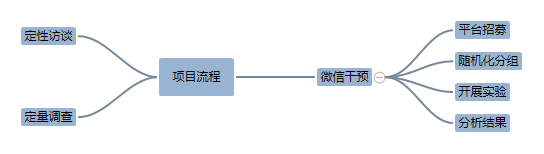
\includegraphics[width=\textwidth]{newprocess.png}
	\centering
	\caption{项目设计简图}
\end{figure}
\subsection{设计创新}
目前的知信行研究仅仅测量干预前效果和干预后的结果,并对这一结果进行直接对比,没有阐释知识、信念、行为之间变化的机制。
为了探索机制(mechanisms)我们需要更多可以观测的变量,和一套可以容纳这些变量的系统。微信公众平台的一系列功能符合
我们的设想。

在同样使用微信公众平台进行知信行研究的案例中,研究者仅仅使用了微信平台发消息的功能,而对于平台搜集的信息没能进行
很好的利用。同时也没有利用投票功能获得期间的反馈,来进行对于过程的控制。
微信公众平台不仅是消息发送的平台,同时具有一定程度的互动功能,同时微信平台提供了丰富的接口可以为知信行模式研究
提供更多可供研究的变量。

zero-cost variable
能够几乎零成本的增加研究的人数,和实验室研究相比成本会降低很多,和现实中的田野研究
相比,能够扩大调查范围。

更多时间分析相关的变量加入:地理信息、终端设备、阅读数、人数追踪。